%%%%%%%%%%%%%%%%%%%%%%%%%%%%%%%%%%%%%%%%%%%%%%%%%%%%%%%%%%%%%%%%%%%%%%%%%%%%%%
\chapter{Discussion} \label{chap:maindisc}
Chapters~\ref{chap:method} through~\ref{chap:behavemodel} presented the experimental approach and evaluations undertaken in seeking to support the thesis for this work:

\begin{quote}
\textit{A robot with \gls{tailored} social behaviour will positively influence the outcomes of tutoring interactions with children and consequently lead to an increase in child \gls{learning} when compared to a robot without this social behaviour.}
\end{quote}

This chapter will present a discussion that draws on the evaluations conducted in the previous chapters and their findings as well as some of the issues introduced in the early chapters of this document. Limitations in the approach adopted here will be outlined, and the discussion will be broadened to show how the work conducted here fits into the larger field of social \acrshort{hri}. Specifically, societal acceptance\footnote{some of this section has been published by the author in \citep{kennedy2016cautious}} and ethical considerations will be explored. The chapter will conclude with suggestions for further research that could build on the findings from this thesis.

%%%%%%%%%%%%%%%%%%%%%%%%%%%%%%%%%%%%%%%%%%%%%%%%%%%%%%%%%%%%%%%%%%%%%%%%%%%%%%
\section{Experimental Limitations} \label{sec:disc-limitations}
This section seeks to acknowledge the limitations in the experimental work conducted throughout this thesis. These limitations stem from various aspects: some theoretical, some practical. These factors must be considered when interpreting the outcomes of this thesis, but they are also used to highlight areas where future work could be performed to further support the findings here (elaborated on in Section~\ref{sec:conc-futurework}).

\subsection{Ecological Validity and Generalisability} \label{sec:disc-experiments}
Several aspects of the experimental design limit the potential generalisability of the findings from this thesis. The first of these limitations is due to a necessary compromise between experimental control and perfect ecological validity \citep{ros2011child}. The experiments are all conducted ``in the wild'', i.e., in the environment of children (their schools). However, the experiments take place outside of the children's normal classroom and instead in other classrooms, or communal spaces. This was done to achieve a certain degree of experimental control (such as preventing other children from overhearing material and therefore being exposed to the material multiple times). This decision may also have led to different behaviour, and subsequently \gls{learning} outcomes, from the children than would have been observed had the robot been present in the normal classroom with other children. Whilst this design choice may have inhibited the confidence of generalisability of results, it is useful to have evidence for effects in relatively controlled environments so that expectations can be formed for classroom use, and so that robot behaviours can be iteratively designed for this environment.

The subject numbers are relatively low for studies which consider human psychology. Typically, a psychology study aims for at least 30 participants to be considered `large', although this approach has been the subject of criticism as it over-simplifies a complex decision \citep{kar201330}. A number of studies undertaken here have around 10-15 subjects per condition (Chapters \ref{chap:embodiment}, \ref{chap:socasoc}, \ref{chap:nviexperiment} and \ref{chap:behavemodel}), which is fairly typical for child-robot interaction studies in the educational domain  \citep{leite2014empathic,saerbeck2010expressive,zaga2015effect}. Nonetheless, from a psychology perspective, this would mean that they would be judged `small' studies, and as such, confidence in the accuracy of the statistical analysis would be reduced. To this end, descriptive statistics, such as confidence intervals, have been included for all studies within this document so that the results do not rely purely on significance testing (as recommended in \citealp{baxter2016althri}).

However, the context of the study should also be considered when deciding on and reviewing sample sizes. Throughout this work, sample sizes have typically been determined by school class sizes. In the U.K., classes range from around 20 to 30 students, so this is used as the total number of participants in many of the studies. Variation between schools, and indeed different classes within schools has the potential to introduce confounds. These confounds can be not just prior knowledge, which could be controlled for, but exposure to different learning styles, or teachers influencing expectations in different ways. Teachers often used interacting with the robot as an incentive to aid classroom management, for example ``be quiet, or you won't get to play with the robot''. Through doing this, the teacher gives importance to the robot and creates expectations which can shape the interaction \citep{fischer2014initiating}. Using a single class as a sample means that the children's expectations will have been shaped in a constant way by a single teacher, thereby providing tighter experimental control in spite of lower subject numbers \citep{baxter2015wider}.

All of the experiments conducted as part of this thesis involved children who had not previously been exposed to the NAO robot. This was an intentional design decision, to ensure that children's expectations would not have been shaped by prior interactions. This allows a comparison between different conditions without having to consider how previous interactions may have influenced behavioural responses. However, longitudinal studies whereby the children were exposed to the same robot multiple times were not conducted. It is entirely possible that many of the observations were due to a novelty effect, where the children were interested in the robot due to its novelty, as opposed to its behaviour, and subsequently responded in a manner that would not be observed in the long-term. Such effects have been suggested to be responsible for observations in other studies, for example \citet{kanda2004interactive,sung2009robots}. The methodology adopted in Chapter \ref{chap:verbal} re-tested children on their \gls{learning} some time after the interaction, thereby verifying that the \gls{learning} was lasting. The work here goes some way to providing design principles for robot behaviour in educational interactions, but exploration of whether \gls{learning} effects persist over longer-term interactions with this behaviour remains to be explored. In any case, the evidence here suggests that short-term interactions do cause \gls{learning}, which could be exploited regardless of whether \gls{learning} gains are observed in prolonged interactions.

\subsection{Measures of Learning} \label{sec:disc-measures}
As stated in the background for this work (Chapter \ref{chap:background}), when measuring a child's application of acquired skills, the measurement may not be of their \gls{learning}, but their performance in the task \citep{mikulas1977learning}. These are complex concepts to disentangle, and so no distinction was made in the experimental work undertaken here. Consequently, improvements in task performance may not have been due to \gls{learning}, but instead because of greater motivation, or children becoming more comfortable over the course of an interaction. However, these factors are constant between conditions, and control conditions with no learning content are also often used in the experiments here. This provides some confidence that what is being measured is in fact child \gls{learning}.

The measures of child \gls{learning} focussed on here were cognitive \gls{learning} gains. This is in part due to the easy collection and good reliability of such data. It is comparatively straightforward to administer pre-tests and post-tests, and to compare scores, as opposed to attempting to collect reliable data on affective \gls{learning} from children, or to monitor the underlying \gls{learning} processes of children. Many affective \gls{learning} measures involve surveys with challenging or irrelevant questions for children of this age, e.g., ``likelihood of taking future courses in this area'' \citep{mccroskey1994assessment}. Whilst these affective aspects of \gls{learning} were not within the scope of the research programme undertaken here, it would nonetheless be worthwhile for future research to pursue this topic to broaden studies on the relationship between robot behaviour and child \gls{learning}.

\subsection{Robot Platform} \label{sec:disc-platform}
The Aldebaran NAO is the only robot platform used in the research conducted throughout this thesis. Whilst the use of just one robotic platform eases comparisons between studies and allows for iterative development of behaviours, it also limits the findings. It is unclear as to whether the observations made here would translate to robots of a different size, appearance, or morphology. In this regard, the results could be somewhat platform specific. However, the findings here do seem to agree with research being conducted in the same domain with different robots.

The NAO robot does not provide the ability to manipulate some of the social cues under consideration in the \acrshort{nvi} measure. For example, the robot cannot produce facial expressions, so it cannot smile. This does not mean that people will not perceive the robot to smile, but it does prevent explicit manipulation of this cue. It may be that greater \gls{learning} effects would be observed if a robot capable of producing facial expressions were to be used, due to the relationship between smiling and \gls{learning} \citep{wilson2007immediacy}, and robot facial expressions and child enjoyment of interactions \citep{cameron2015presence}. The model proposed in Chapter~\ref{chap:behavemodel} proposes that the congruency of social cues is important in the learning outcomes. As such, it would be preferable to work with a platform capable of social cue manipulation along all items of the nonverbal immediacy measure. Currently, there are a limited number of commercially available robotic platforms that would offer all of the necessary affordances to achieve this. When considering robots that would be an appropriate size to use with children, the NAO remains a strong choice despite the lack of ability to produces facial expressions. This may change as an increasing number of robot manufacturers start to use screens as faces, preventing complications with actuating a face in a confined space.

The NAO robot also has relatively loud motors. This could be a factor in some of the findings throughout the thesis, particularly when considering social responses as a product of embodiment. In Chapter~\ref{chap:embodiment}, a physical robot was compared with a virtual one on a screen. When the physical robot moves, the motors could attract attention due to the noise, which would not be the case for the virtual robot. Consequently, children may have looked at the robot more due to the noise (although this also could have been due to the forward motion of the physical robot, that would not be present with the virtual on-screen robot). The motor noise could also have played a role in Chapter~\ref{chap:nviexperiment}, where the robot in one condition moved more than the other condition. If a robot with less motor noise were to be used, it may be that some of the effects between embodiments are no longer as prominent. On the other hand, learning may actually increase. The robot would often be programmed to perform gestures whilst explaining topics (in an aim to be appropriately social), but the motor noise that this introduces may hinder the children's understanding of the verbal content. Without the motor noise, child understanding, and subsequent learning, may improve.

Due to the current wide availability and common use of the Aldebaran NAO, the findings in this thesis are still directly relevant to many other researchers regardless of whether the results generalise to other platforms. The immediacy construct and measurements also provide a framework enabling other researchers to compare other platforms and behaviours against the results found here. Investigation of social behaviour implemented on other platforms characterised through immediacy would certainly provide an interesting avenue for future work.

%%%%%%%%%%%%%%%%%%%%%%%%%%%%%%%%%%%%%%%%%%%%%%%%%%%%%%%%%%%%%%%%%%%%%%%%%%%%%%
\section{Ethical Questions} \label{sec:ch10-ethics}
Chapter~\ref{chap:method} introduced some issues of ethics from a practical perspective. Of course, ethical issues relate not just to practical execution of experiments, but to a wider set of considerations pertaining to whether robots are suitable for use in education at all. \citet{serholt2016classroom} highlight four areas of concern following focus groups with 77 educators in three countries: child privacy, robot responsibility, long-term impact on the child, and accountability of robot actions. These four areas will therefore form the framework for the discussion in this section.

Privacy is recognised as a major ethical concern in relation to robots; partially because robots are commonly used to actively perform surveillance tasks \citep{calo2011privacy}. These concerns change in focus when robots become social companions. \citet{lee2011understanding} suggest that this is due in part to the tendency of humans to anthropomorphise, and the increased likelihood of robots being shared when compared to other technology. Anthropomorphism could cause humans to reveal more information, whilst the shared aspect presents greater opportunity for the spread of the information. People are not fully comfortable with revealing personal information to a robot that it may store, but do see it as a ``necessary evil'' provided that there is a benefit to the user \citep{syrdal2007he}. A reluctance to reveal personal information due to perceptions of sociality could make social robots unsuitable for some applications where the information is critical in forming an appropriate response, or where perceptions of being judged socially may lead to negative behaviours (and indeed where less-social agents may bring about benefits; \citealp{howley2014effects}).

When applied to social robots in education, it is noted by \citet{serholt2016classroom}, that child privacy is a wider concern in education already, with teachers collecting a variety of data about children without their permission. Indeed, the U.K. Department for Education's suggested privacy notice text \citep{dofe2016privacy} includes collecting pupil data to: support learning, monitor and report progress, provide pastoral care, and assess the quality of teaching services. This can include personal characteristics, as well as learning data. Children are not given a choice as to whether they wish to opt out of this data collection. Robots are unlikely to extract any more information than this, however the data is (currently) more likely to be sent to a third party, whereas data at present is kept internally within schools. Striking a balance between privacy and the robot having enough information to be effective, along with whom may access this data, will be an important step in establishing how such technology can be used in an ethically responsible manner in schools.

The role, and associated expectations and responsibilities of robots in schools must be carefully managed. There have long been calls for education to keep up with the pace of technological development (arguably before some of the more impactful technological advances had become commonplace in society; \citealp{will1986educating}). However, there is a distinction between delivering content that educates about technology, and technology that delivers other learning content, although these aspects could of course be intertwined. When technology delivers content, there is a risk that supervising humans do not thoroughly understand the limitations, or the limitations are not immediately apparent. As a consequence, there is a greater chance that it will be used in an unintended manner, with negative cognitive or affective outcomes. While this is in part the fault of the human who employed the technology in that role, the purveyors of the technology must also take some responsibility if limitations are not made clear \citep{johnson2005computer}. It is argued that the temptation to consider technology as ``natural'' must be resisted to prevent undesired moral actions being taken with technology \citep{johnson2005computer}. Clearly in the case of social robots, this temptation is exacerbated due to the precise aim of making the technology more natural in some manner \citep{breazeal2002designing}, combined with the human tendency to anthropomorphise. Limitations of social robots for education should therefore be well documented and portrayed such that the technology is used appropriately.

As part of using social robots in an appropriate manner and to portray limitations accurately, it is necessary to establish the effects not only in terms of \gls{learning} (as explored in this thesis), but also in terms of social well-being. This should be done both at an individual level, and also at a societal level; current decisions about technology can have an impact on future generations, and these temporally ethical decisions must be respected \citep{groves2006technological}. Future research should strive to identify and address long-term risks and benefits of exposure to social robots in general, as well as the case of educative robots in specific. Inspiration can be taken from research of current pervasive technologies such as mobile phones \citep{kamibeppu2005impact} and the Internet \citep{beranuy2009problematic}, but the social aspects and implications need to be explored further due to the social nature of the robots being developed.

The accountability of robot actions is part of an ongoing larger ethical and legal debate surrounding machine autonomy (currently often related to autonomous vehicles as they begin to reach the mass-market; \citealp{beiker2012legal}). Questions of whether the programmer, or the user, are at fault for negative outcomes are often debated, with further complexities in cases where learning algorithms are employed \citep{ros2011child}. It has been suggested that legal frameworks will need to be created on an application-by-application basis \citep{bertolini2013robots}, which presents an opportunity for research into educative social robotics to contribute to the legal debate. Decisions made in this regard will no doubt shape the future of what research may be possible or encouraged.

%%%%%%%%%%%%%%%%%%%%%%%%%%%%%%%%%%%%%%%%%%%%%%%%%%%%%%%%%%%%%%%%%%%%%%%%%%%%%%
\section{Educator and Societal Acceptability} \label{sec:ch10-accept}
Whilst the work conducted here was carried out with the support of schools, there are broader questions of whether robots in education are acceptable to teachers, and society at large. This section seeks to explore some of these areas, also highlighting how the work conducted here might contribute to these larger issues.

As this field of research pushes forwards, and if we seek further real-world or mass-market implementation in schools, it is important to understand attitudes towards the technology. For successful adoption of such technologies, it is necessary for both teachers and the general public to be willing participants in increased uptake. Recent findings from the Eurobarometer report~\citep{eurobarometer2012robots} have suggested that whilst there is generally a positive view towards robots in Europe, there is a sizeable contingent (34\%) that would see robots banned from use in education. However, the survey administered in this report does not provide a context for many of the questions, calling into contention how well-understood or known the kind of social robots that would be used in this domain were for the respondents.

Research has suggested that there are barriers to adoption and use of technology by teachers. These can be first-order (extrinsic) barriers, or second-order (personal) barriers. While the extrinsic barriers cannot be discounted, it has been found that positive beliefs of teachers about the effectiveness for \gls{learning} (i.e., personal factors) are a significant predictor of actual technology use~\citep{blackwell2013adoption}. For this reason, it is important to understand (and possibly influence) how teachers feel towards social robots if we intend to see them widely adopted.

Previous pan-European work~\citep{serholt2014teachers} found that views of teachers are generally positive, but that there are concerns over fairness to access, the robustness of the technology, and potential disruption to classrooms. Some of these same concerns were observed prior to an experiment in the USA, but after the experiment had been completed, views had changed~\citep{kory2016lessons}. Teachers expected the robot to be disruptive to the classroom, but found that it was not, although this is partially mitigated as headphones were used so that the possibility of audible disruption would be minimised. A large-scale survey conducted in South Korea~\citep{lee2008elementary} found that teachers were generally positive about the use of robots in education, but they were more negative than other stakeholders.

When exposed to a highly scripted interaction with a robot, teachers showed fairly positive reactions~\citep{fridin2014acceptance}, however it was concluded that the interaction here was not related to the educational quality that the robot could offer, and this is where the focus should be. Incorporating the views of teachers in educational technology design has been highlighted as a particularly important aspect of creating a partnership that allows teachers to identify the benefits and shortcomings of technology when related to the curriculum~\citep{okita2011current}. 

Revisiting \citet{serholt2016classroom}, the long-term impact of educative robots on children was raised as one of four central issues following focus groups with 77 educators in three countries. Long-term consideration of children's welfare has been raised as an issue in other studies as well. \citet{kennedy2016cautious} finds that educators concerns about appropriate long-term social skills for the robots dominate over practical and ethical concerns. These social skills involve the richness of the interaction, the adaptability of the robots to change in response to child behaviours, or the suitability of social robots to develop children's peer-group sociality, all of which present fundamental questions for research in this field. It is therefore suggested that these behavioural considerations must remain central to the research agenda of child-robot interaction \citep{kennedy2016cautious}, but that we progress bearing in mind the responsibility we have to children \citep{serholt2016classroom}.

Due to the technological nature of robots, it is reasonable to hypothesise that they will be seen as a tool for STEM education, rather than for the teaching of humanities. This is reflected in the research being conducted with robots in education: they are commonly applied in STEM education, with promising outcomes \cite{karim2015review}, although research is also prominent in language contexts \cite{hood2015children,kanda2004interactive,kennedy2016social,tanaka2012children}. However, there are comparatively few robots being used to teach art or religious education, for instance (a reference to work in either of these domains could not be identified at the time of writing). Some perceptions based on pre-conceptions may well change with greater exposure to social robots that can do more than be used as a tool for STEM subjects (for example, as recently shown with handwriting learning;~\citealp{hood2015children}). This is potentially where the broader aspects of using a social robot could be beneficial in breaking down some barriers to use. The robot is a technological device, but could be used to teach a variety of subjects with an element of sociality. The use of the robot could stimulate interest in technology, and the social aspects of robot behaviour could be used to create reciprocal interest in those subjects (as has been attempted for some aspects of behaviour;~\citealp{gordon2015curiosity}). This calls for a greater exposure of teachers to our robotic systems, so that they better comprehend the capabilities, current limited performance, and possible future applications of social robots in education. The efficacy of such applications must also be clearly demonstrated.

Successfully addressing the concerns highlighted by educators in the various studies would provide an essential first step towards achieving greater adoption (if indeed this is desirable). Some of the concerns may arguably be alleviated once the teachers and the children familiarise themselves with the robots (the robot being a source of distraction is likely to resolve quickly after novelty goes away) or once the penetration of robots in classrooms increases to a point where dedicated companies could regularly take over training and maintenance issues. Overall, the attitude towards social robots in schools is potentially accepting \citep{lee2008elementary,serholt2014teachers}. For the educators, concerns about appropriate social skills for the robots are raised in addition to the practical and ethical concerns. The work in this thesis contributes in some part to addressing concerns regarding social capabilities of such robots, but this should remain a focus for child-robot interaction research as more work is required to explore longer-term impacts on children interacting regularly with social robots.

%%%%%%%%%%%%%%%%%%%%%%%%%%%%%%%%%%%%%%%%%%%%%%%%%%%%%%%%%%%%%%%%%%%%%%%%%%%%%%
\section{Sociality and Learning} \label{sec:ch10-social}
The thesis put forward here centres around \textit{social behaviour} and \textit{\gls{learning}}, and in particular, the connection between these concepts. This section seeks to critically discuss the approach to social behaviour and \gls{learning} in the work carried out, as well as to consider the three predictions generated from the model created in Section \ref{sec:chap9-nonvlearn} in a broader context.

As identified in the background (Chapter~\ref{chap:background}), acquiring data from children regarding their subjective perceptions of an interaction and robot behaviour is particularly challenging. To minimise the problems in acquiring such data, \gls{nonverbalimm} was used, which considers only overt social cues. Chapter~\ref{chap:validation} demonstrated the validity of this approach, but it is still not without limitations, as highlighted in Chapter~\ref{chap:behavemodel}.

While \gls{nonverbalimm} provides a characterisation of robot behaviour as perceived by children, it does not describe the relationship they feel towards the robot, or their perception of the social aspects of the interaction as a whole. In the studies conducted here, additional questions were commonly added to the end of questionnaires that were administered, but these gave an indication of the relationship felt by the children, rather than exploring it in detail. For example, ``For me, I think the robot was like a - ...'', as seen in Appendix \ref{app:rrq}. Greater \gls{nonverbalimm} has been correlated with increased friendliness \citep{wilson2007immediacy}, but children did not (statistically) consistently report robot conditions with higher \gls{nonverbalimm} to be more like a friend. Of course, increased friendliness would not necessarily lead to children relating to the robot as a `friend', but given the limited data collected here this would provide the best indicator. It would be desirable to explore the relationship between the child and the robot in greater detail to better understand the interaction from the child's perspective. This could reveal areas for further improvement in the robot social behaviour. However, this is an extremely challenging task, with no straightforward solution to implement when conducting studies with reasonably high numbers of children. Structured interviews could be valuable, but are incredibly time consuming when dealing with tens of young subjects, who are likely nearing their attention limit after interacting with the robot.

Specific aspects of \gls{learning} were the focus of the research here. Figure~\ref{fig:ch10-learningtaxonomy} has been reproduced from Chapter~\ref{chap:background}, which indicates where the focus of learning was. It is in the cognitive domain, and it is clear that a large area of the taxonomy is not addressed. Nor is the affective domain addressed -- that is not to say it was not influenced in the work here, but measuring and accounting for any change in this domain was not within the scope of the work (Section~\ref{sec:intro-scope}). This is not uncommon in the field of \acrshort{hri} research, with many studies exploring `remember' \citep{alemi2014employing,szafir2012pay}, `understand' \citep{kory2014storytelling,tanaka2012children}, or `apply' \citep{leyzberg2014personalizing} cognitive processes. Relatively few studies consider meta-cognitive analysis, evaluation, or creation. This may in part be due to the additional complexity in scenario and knowledge interpretation/representation that would be required either automatically from robot sensors, or to be input by a Wizard.

\begin{figure}[h]
    \centering
    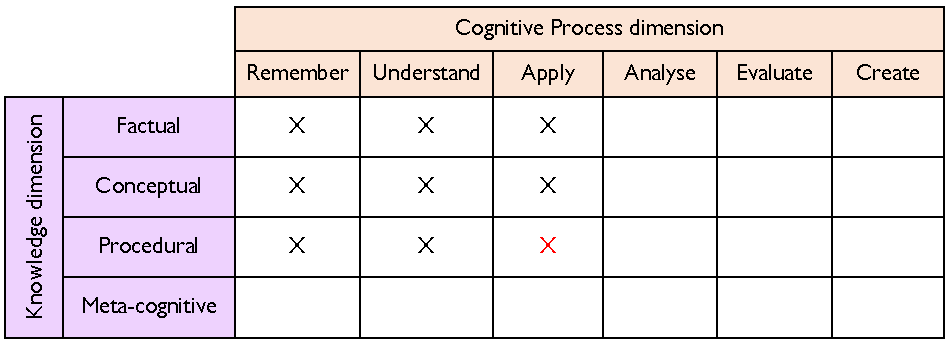
\includegraphics[width=0.75\textwidth]{images/ch2_LearningTaxonomy.pdf}
    \caption{The revised educational objectives `Taxonomy Table' (adapted from \citealp{krathwohl2002revision}). Crosses indicate the areas focused on in studies throughout the research here, with the red cross signifying the intersection at which performance is most often measured. Reproduced from Chapter~\ref{chap:background}.}
    \label{fig:ch10-learningtaxonomy}
\end{figure}

In Chapter~\ref{chap:behavemodel}, a model was proposed that made three predictions for the relationship between sociality and \gls{learning}. To explore these further, other literature will be considered in the context of the predictions, which will also tie back to the background from Chapter~\ref{chap:background} (specifically Section \ref{sec:background-robottutors}), where a mixed picture was discovered in the relationship between social behaviour and \gls{learning}. As a reminder, the predictions of the model were as follows:
\begin{enumerate}
	\item [P1.] Highly social behaviour of a tutor robot (as characterised by \gls{nonverbalimm}) with high congruency will lead to maximum potential \gls{learning}.
	\item [P2.] Low social behaviour of a tutor robot with low congruency will lead to minimal potential \gls{learning}.
	\item [P3.] A mismatch in the social behaviour of a tutor robot and the social cue congruency will lead to less than maximum potential \gls{learning}.
\end{enumerate}

Prediction 1 suggests that highly social behaviour with high congruency will lead to maximum potential \gls{learning}, and prediction~2 is the inverse of this. The former could be demonstrated through \citet{saerbeck2010expressive}, where a number of social cues were modified in unison, including gestures, verbal utterances and emotional expressions. As such, it could be suggested that the cues are both highly social and congruent, explaining the improvement in \gls{learning} that is shown when compared to a robot without these behaviours. \citet{herberg2015robot} may have experienced unexpected results because the robot did not employ many social cues (there are no gestures, body posture changes, or facial expressions, for example), but then one condition has more animated gaze than the other condition. Through adding this gaze, the cues are not only minimally social, but now also incongruent (as one cue is social whilst the others are not utilised), leading to less \gls{learning} than the robot without this additional gaze cue (which therefore has low social cue use, but with more congruency), demonstrating prediction~2. Prediction 3 could explain the results of \citet{kanda2012children}, where increased social behaviour was operationalised only through verbal utterances and no \gls{learning} differences were observed. Although the addition of verbal utterances increased the social behaviour, it simultaneously reduced the congruency (as no other cues were made more social), leading to no change in \gls{learning}.

It is acknowledged that these predictions are made based on the framework of the data generated from this thesis, which as this section has discussed, only considers a sub-set of the expanse of how both \gls{learning} and social behaviour may be defined. This does not necessarily detract from the model, or the possible validity of the predictions, but instead highlights the current challenges in this relatively new domain and the need for further exploration. Fully understanding how to teach using machines is a long-studied, and ongoing field of research, with the recent addition of robots introducing additional unanswered questions \citep{timms2016letting}. Characterising and understanding social behaviour is also a complex task, with research in neuroscience and psychology still not providing an account for these aspects. It is becoming recognised that models of unified behaviour may be required \citep{zaki2013cue}, with a broad set of social behaviours incorporated (including affective components alongside social cues and social-cognitive functions; \citealp{pfeiffer2013gaze}). Restricting the focus of \gls{learning} and social behaviour therefore becomes a more tractable approach to establish models to build from given the quantity of unknowns in the exploration. However, there is clearly a need to build increasingly comprehensive models for generating and understanding social behaviour for robots once more basic principles have been rigorously established; this is highlighted as future work in the subsequent section.

%%%%%%%%%%%%%%%%%%%%%%%%%%%%%%%%%%%%%%%%%%%%%%%%%%%%%%%%%%%%%%%%%%%%%%%%%%
\section{Comparisons Between Children and Adults}
Much of the work conducted in this thesis has been influenced by findings from human-human literature with adults, in particular the use of immediacy, which is commonly applied in university lecture contexts \citep{witt2004meta}. Additionally, the quantity of similar work focussing on learning and social behaviour in the field of human-robot interaction applied to child tutoring, while increasing, is not sufficient to provide a thorough background for the work here. As such, comparisons were often made between results found with children and results found with adults, and experiments would be explicitly designed in a manner that attempted to tie findings between human adults to HRI scenarios with children (for example, Chapter~\ref{chap:validation}). This section seeks to draw on this experience to discuss the merits of such comparisons.

When attempting to apply the concepts and adapt the measures used in nonverbal immediacy for use with children, many issues arose in terms of the language used in the original questionnaires as they had been designed for adults. This was an even greater problem in other questionnaire series, with common use of abstract terms, e.g., \citet{bartneck2009godspeed}. This lead to an adaptation of nonverbal immediacy being used. Challenges then arise because the metric is no longer the one previously validated with adults, and children are known to interpret and complete questionnaires in a different manner to adults in any case \citep{belpaeme2013child,borgers2000children,borgers2004response}. For this reason, adults were used as a baseline in the initial validation of the adapted scale performed in Chapter~\ref{chap:validation}. However, when comparing the child and adult perceptions according to the scale, whilst the ranking was the same and the correlation was strong, the children were clearly far more tightly bunched in their scores. This could be due to a tendency for children to score highly on questionnaires, or it could be a genuine difference in perceptions. This would not be surprising, given that children are still establishing social behavioural norms and learning to process social information \citep{bandura1963social}. Indeed, it may be the case that children focus on different social features to adults while they develop concepts of social behaviour from salient cultural practices \citep{whiting1992children}. For this reason, the comparison between child and adult perceptions may not be particularly worthwhile. Although the adult results provide some context, they do not necessarily help to understand the perspective of the child.

Due to the relative lack of other research in the field of social HRI exploring robots for tutoring, many hypotheses and experiments were derived from results acquired with adults. As an example, Chapter~\ref{chap:embodiment} sought to address issues of embodiment and drew on findings from \citet{bartneck2003interacting} and \citet{leyzberg2012physical} to motivate the hypothesis that a physically embodied robot would lead to greater child learning. This was not found to be the case, in agreement with other work conducted with children using a similar methodology (the same robot on a screen vs. physically present; \citealp{looije2012help}). Consequently, the findings appear to be unclear: they are in agreement with some work, but not others. It could be a product of subject age that this problem occurs; if only the child results are considered, then it may simply be the case that the embodiment effect is not present. Comparing to the adult results may serve to confuse matters in this instance.

Furthermore, there are limited resources for use with children in terms of holistic metrics for social behaviour, an issue that is exacerbated when looking specifically for measures that might work with robots. There are currently also limited publications in the field of HRI using children as subjects (although recently this appears to be changing; \citealp{HRI2017hri}). This creates a challenge when attempting to base experimental work in the context of prior literature. It is suggested here that when the subject group changes from children to adults, comparisons with prior literature has limited utility as age will always serve as a confound. As such, it would seem prudent for those working with children to focus on developing more tools and findings specifically for this age group (or possibly age groups, splitting by developmental stage). Such an approach would provide a more satisfactory context for future work and possibly assist in creating a more coherent body of literature, an issue highlighted in Chapter~\ref{chap:background}.


%%%%%%%%%%%%%%%%%%%%%%%%%%%%%%%%%%%%%%%%%%%%%%%%%%%%%%%%%%%%%%%%%%%%%%%%%%
\section{Future Work}\label{sec:conc-futurework}
The work conducted in this thesis has clearly highlighted the potential for the use of robots as tutors for children, and the educational value of tailoring robot social behaviour with the aim of improving \gls{learning} outcomes. It should be made clear, however, that there remain many open questions for such applications, either because they fell outside the scope of the research conducted here, or because of current limitations in social robotics. This section picks up from many threads of the discussion above, and from Chapter~\ref{chap:behavemodel}, outlining possible future research directions that may provide further value and insight for the design of robot tutors for children.

\subsection{Building on the Social Cue and Congruency Model}
Chapter~\ref{chap:behavemodel} proposed a model for the explanation of child \gls{learning} as a product of social cues and cue congruency. Future work could seek to explore this model and extend or revise it where necessary. The work in this thesis used \gls{nonverbalimm} as the characterisation of social cues for the model. As discussed in Chapter~\ref{chap:behavemodel}, the indicator of cue congruency, Guttman's G6 across the \gls{nonverbalimm} items is likely an imperfect measure for this purpose. Ideally, to build on the model, a metric for social cue congruency would be developed and validated to provide more confidence in the evaluations for this dimension. It may also be necessary to modify or use an alternate scale for the characterisation of social behaviour as measuring only social cue use might not be sufficient given that the timing of the cues is not evaluated in NVI (as highlighted in Chapter~\ref{chap:behavemodel}).

Regardless of whether the dimensions on the scale are modified or not, the model put forwards in this thesis provides a set of three testable predictions, reproduced below. It would be straightforward to create a set of robot behaviours for each one of these predictions, for example, a robot with high social cue use, and high congruency for P1, and so on. These could then be applied in a variety of learning contexts to validate whether the predictions hold true across contexts given consistent behaviour. The same could be done with a variety of robot hardware platforms to examine the impact of certain cues not being available. Collection of a variety of data in this regard would provide more data points for the proposed model space, and could be used to validate, or revise and improve the model.
\begin{enumerate}
	\item [P1.] Highly social behaviour of a tutor robot (as characterised by \gls{nonverbalimm}) with high congruency will lead to maximum potential \gls{learning}.
	\item [P2.] Low social behaviour of a tutor robot with low congruency will lead to minimal potential \gls{learning}.
	\item [P3.] A mismatch in the social behaviour of a tutor robot and the social cue congruency will lead to less than maximum potential \gls{learning}.
\end{enumerate}

\subsection{Accounting for Individual Differences}
Whilst the robot behaviour in the interactions that took place throughout the experimental studies here were often adaptive to the children in some way (for example, behaviours tracking child gaze, or occurring in response to children moving images on the touchscreen), incorporating greater adaptation into robot social behaviour may lead to further educational, and interaction-quality, advantages. This principle has been demonstrated at a task level \citep{coninx2015towards}, with work in preparation suggesting that the same could apply to lower level social behaviours \citep{baxter2016robot}. However, in order to generate appropriately adaptive behaviours, we need to establish not only a model of child social (and \gls{learning}) responses to robot social behaviour, but to also characterise the child through some means in order to inform any adaptation that takes place. This could be done on-line through adapting to the child's social behaviour, or off-line through responses to personality questionnaires or similar. This is being explored by other researchers in terms of modelling and generating behaviour in response to child knowledge \citep{jones2015open}, affective states \citep{spaulding2016affect}, and behavioural traits \citep{baxter2016robot}. However, work from neuroscience suggests it may be necessary to draw more of these elements together into larger models of social cognition \citep{pfeiffer2013gaze} due to the unified nature of social processing \citep{zaki2013cue}. This is clearly an ambitious path of research due to the scale of the problem, but it presents an opportunity for \acrshort{hri} to contribute to our understanding of human psychology.

\subsection{Increasing Interactivity}
The interactions taking place in this research did not typically involve large elements of verbal interaction. This was due to current limitations in child speech recognition \citep{kennedy2014chatbot}. It is challenging to use speech recognition with children in a robust manner; often this can be circumvented through using a `Wizard' to type in speech, or to perform some part of the cognitive processing to do with language on behalf of the robot \citep{baxter2016althri}. However, this technique can introduce methodological variations and does not accurately reflect current robot abilities, so was not adopted here. Clearly, as speech recognition for children improves, more interaction can take place in the verbal domain, opening further opportunities for research.

Using a different platform to the one used here (the Aldebaran NAO) would also create a useful extension to the current findings. As indicated previously, the Aldebaran NAO is limited in terms of certain social cues, such as facial expressions. It is possible that with the addition of other modalities, the relationship and interactivity with the child may also change. The characterisation of social behaviour through immediacy laid out in this research provides an ideal framework within which this extension could be performed to build on the findings here.

\subsection{The Robot Role}
As stated in Chapter \ref{chap:method}, the aim here was not to replace human tutors, but instead use robots to offer additional opportunities to supplement current human tutoring provision. Robots can assume a wider variety of roles than a human in tutoring. For example, robots can assist teachers \citep{alemi2014employing}, or offer children a chance to teach a less-able peer \citep{tanaka2012children, hood2015children}. Alternatively, robots could provide personalised support which falls outside of typical lessons or the school environment, such as additional language support for non-native children, as discussed in \cite{belpaeme2015L2TOR}. These opportunities typically lend themselves to the one-to-one scenario explored here, but focus on the robot adopting a more peer-like role than the robot often did in the research here. These complementary roles are certainly worth further exploration.

The scope of this work focussed on the relationship between the child and the robot in response to social behaviour, and the impact that this has on the cognitive \gls{learning} that takes place. However, cognitive \gls{learning} is only one aspect of \gls{learning}, with affective \gls{learning} also playing a key role in the pedagogical process \citep{krathwohl1964taxonomy}. The affective domain includes consideration of attitudes towards \gls{learning} and motivation for \gls{learning}, so takes on increasing importance over the longer-term. This is an area which could initially be exploited by any novelty effects that social robots may introduce to \gls{learning}, but further research into longer-term maintenance of both affective and cognitive \gls{learning} effects would be worthwhile; an issue raised by many other researchers, and well summarised in \cite{leite2013social}.

\subsection{Sustained Use and Adoption}
Section~\ref{sec:ch10-accept} raised questions as to whether society and educators will accept educative social robots, and indeed Section~\ref{sec:ch10-ethics} challenges whether this should even be an aim. In both cases, the long-term well-being of children who interact for sustained periods with social robots appears to be of utmost importance. As such, research should seek to establish the cognitive and socio-emotional effects of long-term interaction with social robots. This must of course be conducted in an ecologically valid manner such that findings can inform decisions made at a societal level as to when and how the robotic technology should be used. It is likely that exploration in this direction will simultaneously require more complex robot behaviour (whether through regular updates to introduce novelty or through models of cognition) to sustain interactions over time. This is a substantial challenge not only for social robots in education, but for social robots more generally \citep{leite2013social}.

%%%%%%%%%%%%%%%%%%%%%%%%%%%%%%%%%%%%%%%%%%%%%%%%%%%%%%%%%%%%%%%%%%%%%%%%%%%%%%
\section{Summary} \label{sec:maindisc-summary}
This chapter outlined limitations in the approaches adopted in the experimental studies conducted throughout this thesis, highlighting the potential impact on the findings, and future avenues for research, where relevant. Additionally, the discussion was broadened to take a wider view of where the program of research undertaken here fits into the field of \acrshort{hri} and society more generally. The ethical implications of such technology were explored through other literature, as was societal and educator acceptance of the technology. From these considerations, it was suggested that further study into the long-term effect of social robots not only on child \gls{learning}, but also their more general well-being should be pursued. To achieve this, improved robot social behaviour may be necessary (along with understanding of how to generate effective social behaviour), as well as an expanded record of efficacy over longer time periods for the educational aspects for the investment to be worthwhile. Many of these challenges will align with problems that the field of \acrshort{hri} is facing generally, but adaptations must be made to tailor findings for the education domain, and often also for children.